\section{Introduction}

You have probably noticed that large speakers for stereo systems have more 
than one actual speaker in them. Some are very big and provide the bass end, 
while others can be quite small, dishing out the higher frequencies. How do 
the electronics inside divide up the total sound signal into low and high 
frequency parts? Here we will find out the answer to this question and many
others. The key component needed for this task is the capacitor.

First we will look at the DC response of a capacitor and find that it 
introduces a new parameter into the circuit that defines a time scale for 
charging and discharging phenomena. This time parameter is called the {\em 
$RC$ time constant}. After thoroughly characterizing the direct current effects
of the capacitor, we will then move on to oscillating circuits; here the 
interesting effects arise from the interplay of the two time scales, one 
associated with the period of the current oscillation and the other with 
the capacitor. This will lead us to the idea of a filter, and then we will 
characterize the two main types of filters, hi-pass and low-pass.

\section{Theory}

\subsection{References}

Serway discusses capacitance in Chapter~26 (Capacitance and Dielectrics), 
within the context of dc circuits. He discusses ac circuits in 
Chapter~33 (Alternating Current Circuits), and specifically capacitors 
in ac circuits in Section~33.4 (Capacitors in an ac Circuit). The ideas
involved in filtering appear in Section~33.8 (Filter Circuits), but we 
will approach the subject from a different perspective. You should glance 
through these sections before proceeding further.

We will also run across some special types of equations, called differential 
equations, that we will need to solve. A good reference for the standard 
techniques is 
\begin{quote}
W. E. Boyce and R. C. DiPrima, {\it Elementary Differential Equations and 
Boundary Value Problems, 4th edition}, J. Wiley \& Sons, New York, 1986.
\end{quote}

\subsection{DC Response of Capacitors}

\begin{figure}[htb]
\centering 
\epsfxsize=10cm 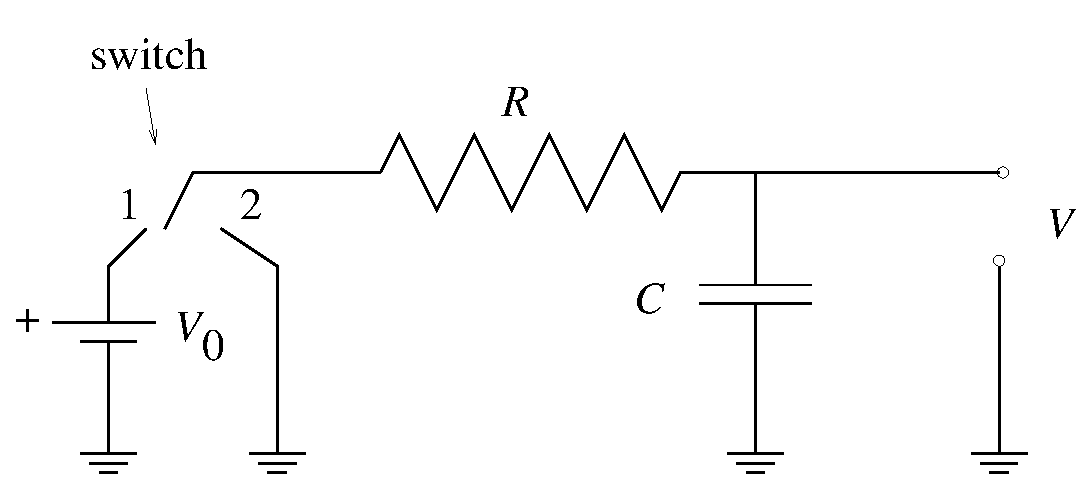
\includegraphics[scale=0.5]{5_rccircuits/rc1.eps}
\caption{The basic DC capacitor circuit.}
\label{fig:RC:cap1}
\end{figure}

Consider the circuit that appears in Figure \ref{fig:RC:cap1} and let the 
switch be in position 1. In this position, the circuit is charging the 
capacitor, since current will flow, carrying positive charge, from the voltage 
source to the capacitor; this will then force positive charges off the other 
plate into ground. Alternatively, electrons (negative charges) flow off of the
top plate of the capacitor to the voltage source and from ground to the bottom
plate; in either way of looking at it, charge builds up on the capacitor. As 
more and more charge accumulates on the plates of the capacitor, it will take 
more and more emf to push charges onto the plates. Thus, we expect this 
process to slow as time continues; {\it i.e.}, the current flowing in the 
circuit should decrease in time. Correspondingly, the voltage across the 
capacitor should approach the emf of the voltage source. Let's see if we can 
quantify this heuristic discussion.

Let the capacitance of the capacitor be $C$ and the resistance of the 
resistor be $R$, with the voltage source generating an emf of $V_0$. We 
want to write down Kirchoff's laws for this circuit. If a current $i$ flows 
through the resistor, then the voltage drop across it is $V_R = iR$. If 
charge $Q$ develops across the capacitor, then the voltage drop across it 
is $V_C=Q/C$. These two voltage drops must add to give the (constant)
emf of the source $V_0$:
\begin{eqnarray*}
V_0=V_R+V_C=iR+\frac{Q}{C}.
\end{eqnarray*}
Recall that the current is simply the time derivative of the charge:
$i = dQ/dt$; inserting this into Kirchoff's law and rearranging 
yields the following first-order, linear, inhomogeneous differential 
equation for the charge on the capacitor:
\begin{eqnarray*}
\frac{dQ}{dt} + \frac{1}{RC}Q = \frac{V_0}{R}.
\end{eqnarray*}
We need to solve this equation for $Q$ as a function of time. Before we
can do this, we must specify an initial condition, {\it i.e.}, we must choose 
what the charge on the capacitor is before we turn the circuit on. The only 
really natural choice is obviously 0, for how could any charge get on the 
plates before we start to charge it! So, we have to solve the initial 
value problem
\begin{eqnarray}
\frac{dQ}{dt} + \frac{1}{RC}Q &=& \frac{V_0}{R},   \label{eq:RC:ode1}\\
Q(0) & = & 0. \nonumber
\end{eqnarray}

There are many techniques for solving linear, first-order differential 
equations. The easiest technique uses what is called an integrating factor. 
The idea behind this technique is to multiply equation (\ref{eq:RC:ode1}) by a 
very carefully chosen function so that the two terms on the left combine into 
the derivative of a product; such a function is called an integrating factor 
for the equation. The integrating factor for our equation is
\begin{eqnarray*}
e^{t/RC};
\end{eqnarray*}
see Boyce and DiPrima for a more general discussion of integrating factors and 
how to find them. Carrying out this procedure, we find
\begin{eqnarray*}
e^{t/RC} \left[\frac{dQ}{dt} + \frac{1}{RC}Q \right] & = & e^{t/RC}\frac{V_0}{R}\\
\frac{d}{dt} \left[ e^{t/RC} Q \right] & = & \frac{V_0}{R}e^{t/RC}.
\end{eqnarray*}
Integrating both sides with respect to $t$ yields
\begin{eqnarray*}
e^{t/RC} Q = CV_0 e^{t/RC} + {\rm const.}
\end{eqnarray*}
from which we find
\begin{eqnarray*}
Q = CV_0 + {\rm const.}e^{-t/\tau}
\end{eqnarray*}
where we have introduced the {\em RC time constant} $\tau = RC$. Notice that
$CV_0$ is just the charge the capacitor would store if the voltage across it 
were $V_0$. Denoting this value by $Q_0$, we can then determine what the 
unknown constant in our equation is by enforcing the condition that $Q=0$ 
when $t=0$. If this is to be true, then the constant must be $-Q_0$ and our
final solution for a charging capacitor is
\begin{eqnarray}
Q(t) = Q_0 (1-e^{-t/\tau}) \label{eq:RC:charging}
\end{eqnarray}

Since we can't measure charge directly, this is not an easy equation to 
verify. We can, however, very easily ascertain the voltage across the 
capacitor. At any time $t$ this voltage is $V(t)=Q(t)/C$; so, we find from 
equation (\ref{eq:RC:charging})
\begin{equation}
V(t) = V_0(1-e^{-t/\tau}), \label{eq:RC:chargingv}
\end{equation}
which we can detect with a multimeter or oscilloscope, if we want. We can also 
determine the time dependence of the current from 
equation~(\ref{eq:RC:charging}) by simply taking the time derivative:
\begin{eqnarray*}
i(t) = \frac{dQ}{dt} = i_0 e^{-t/\tau},
\end{eqnarray*}
where $i_0=Q_0/\tau$. Thus, the voltage starts from $0$ and asymptotically 
approaches $V_0$, while the current begins at $i_0$ and exponentially 
decreases to $0$. In Figure \ref{fig:RC:chargingiv}, we 
graph the voltage and current as functions of time.
\begin{figure}[htb]
\centering 
\epsfxsize=8cm 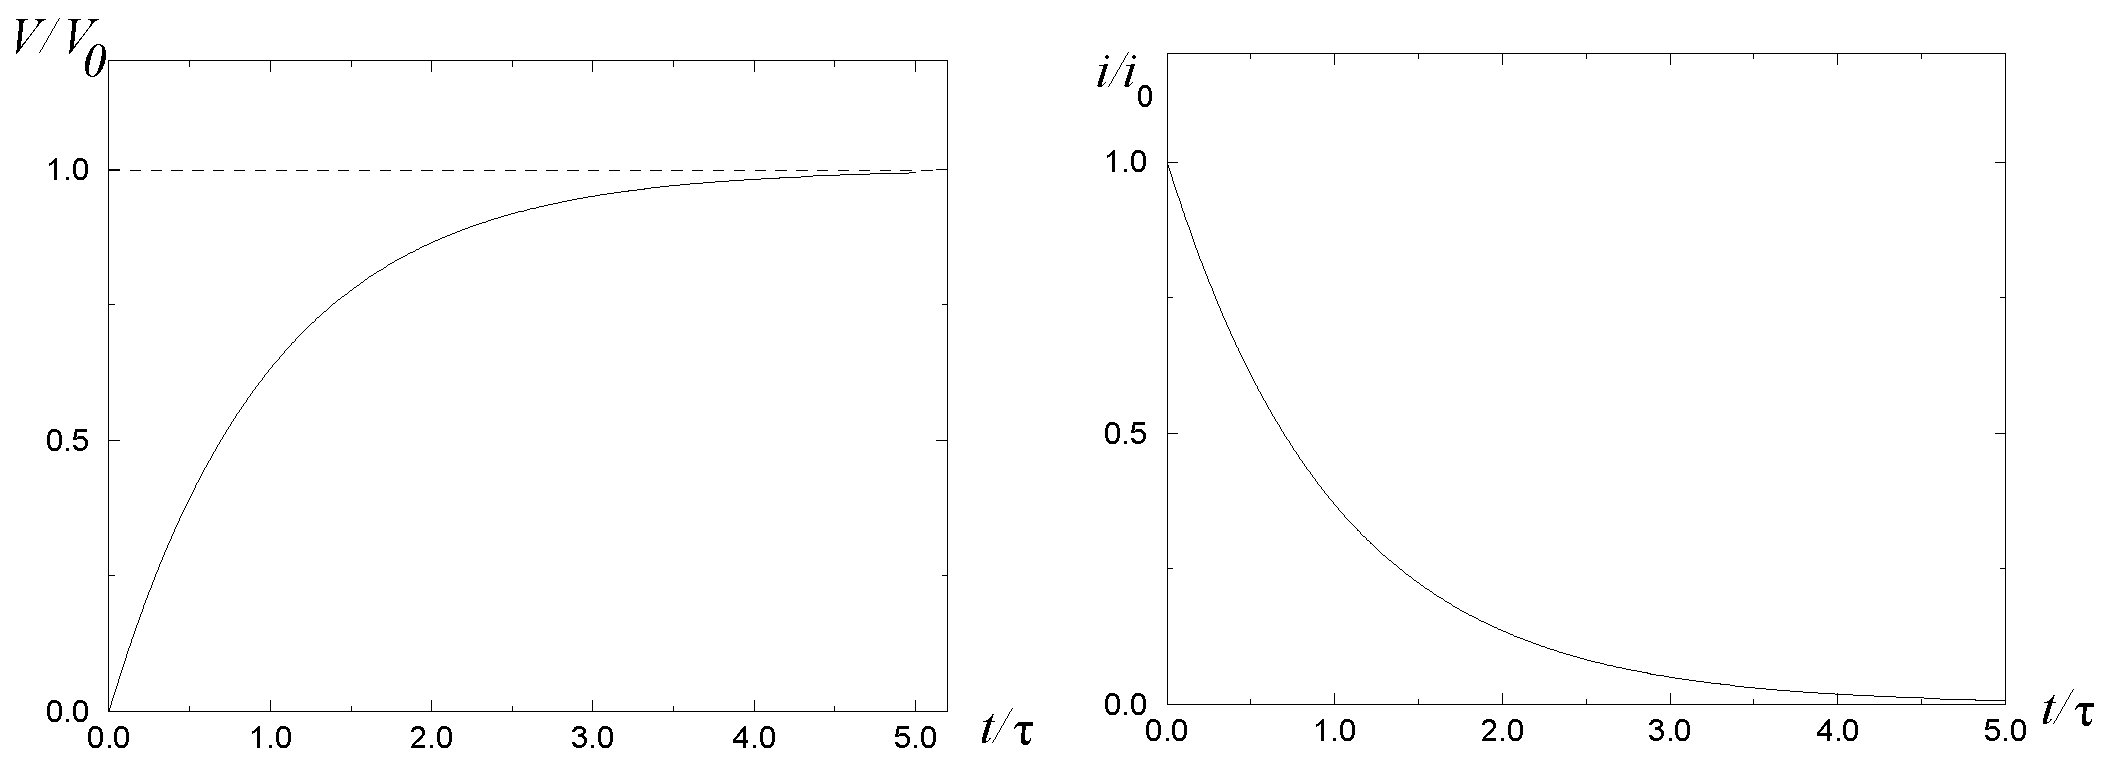
\includegraphics[scale=0.4]{5_rccircuits/chargevi.eps}
\caption{Plots of the voltage across the capacitor and the charging current 
as a functions of time.}
\label{fig:RC:chargingiv}
\end{figure}

Now consider what happens if we move the switch to position 2 in Figure
\ref{fig:RC:cap1}. The capacitor will then discharge through the resistor; how 
do the current and voltage behave as a function of time in this case? We can 
set up the analysis just as we did in the charging case. Applying Kirchoff's 
laws, we find that the voltage drops must sum to zero:
\begin{eqnarray*}
V_C+V_R = \frac{Q}{C} + iR = 0;
\end{eqnarray*}
inserting the definition of current, we find that the charge on the capacitor
obeys the following differential equation:
\begin{eqnarray*}
\frac{dQ}{dt} + \frac{1}{RC}Q = 0,
\end{eqnarray*}
with $Q(0)=Q_0$ the charge on the capacitor after charging. You can solve this
equation by simply separating the variables and integrating:
\begin{eqnarray*}
\int_{Q_0}^{Q} \frac{dQ}{Q} = - \int_0^t \frac{dt}{RC},
\end{eqnarray*}
or 
\begin{eqnarray*}
Q(t) = Q_0 e^{-t/\tau},
\end{eqnarray*}
where $\fbox{$ \displaystyle \tau = RC $}$  is again the time constant of the circuit. Having the charge
as function of time leads us to the voltage and current behavior, just as in 
the previous case:
\begin{eqnarray}
\fbox{$ \displaystyle V(t) = \frac{Q(t)}{C} = V_0 e^{-t/\tau} $} \label{eq:RC:discharge voltage}\\
i(t) = \frac{dQ}{dt} = - i_0 e^{-t/\tau},\nonumber
\end{eqnarray}
where $V_0 = Q_0/C$ and $i_0 = Q_0/\tau$. Notice that the current is negative
here, reflecting the fact that the charge is coming off the capacitor, rather 
than accumulating on it. Also notice that the time dependence is still 
controlled by $\tau$. In Figure \ref{fig:RC:dischargingiv} we graph the 
current and voltage as functions of time. We see from this figure that both 
the voltage and current exponentially decay to zero as the capacitor 
discharges.
\begin{figure}[htb]
\centering 
\epsfxsize=8cm 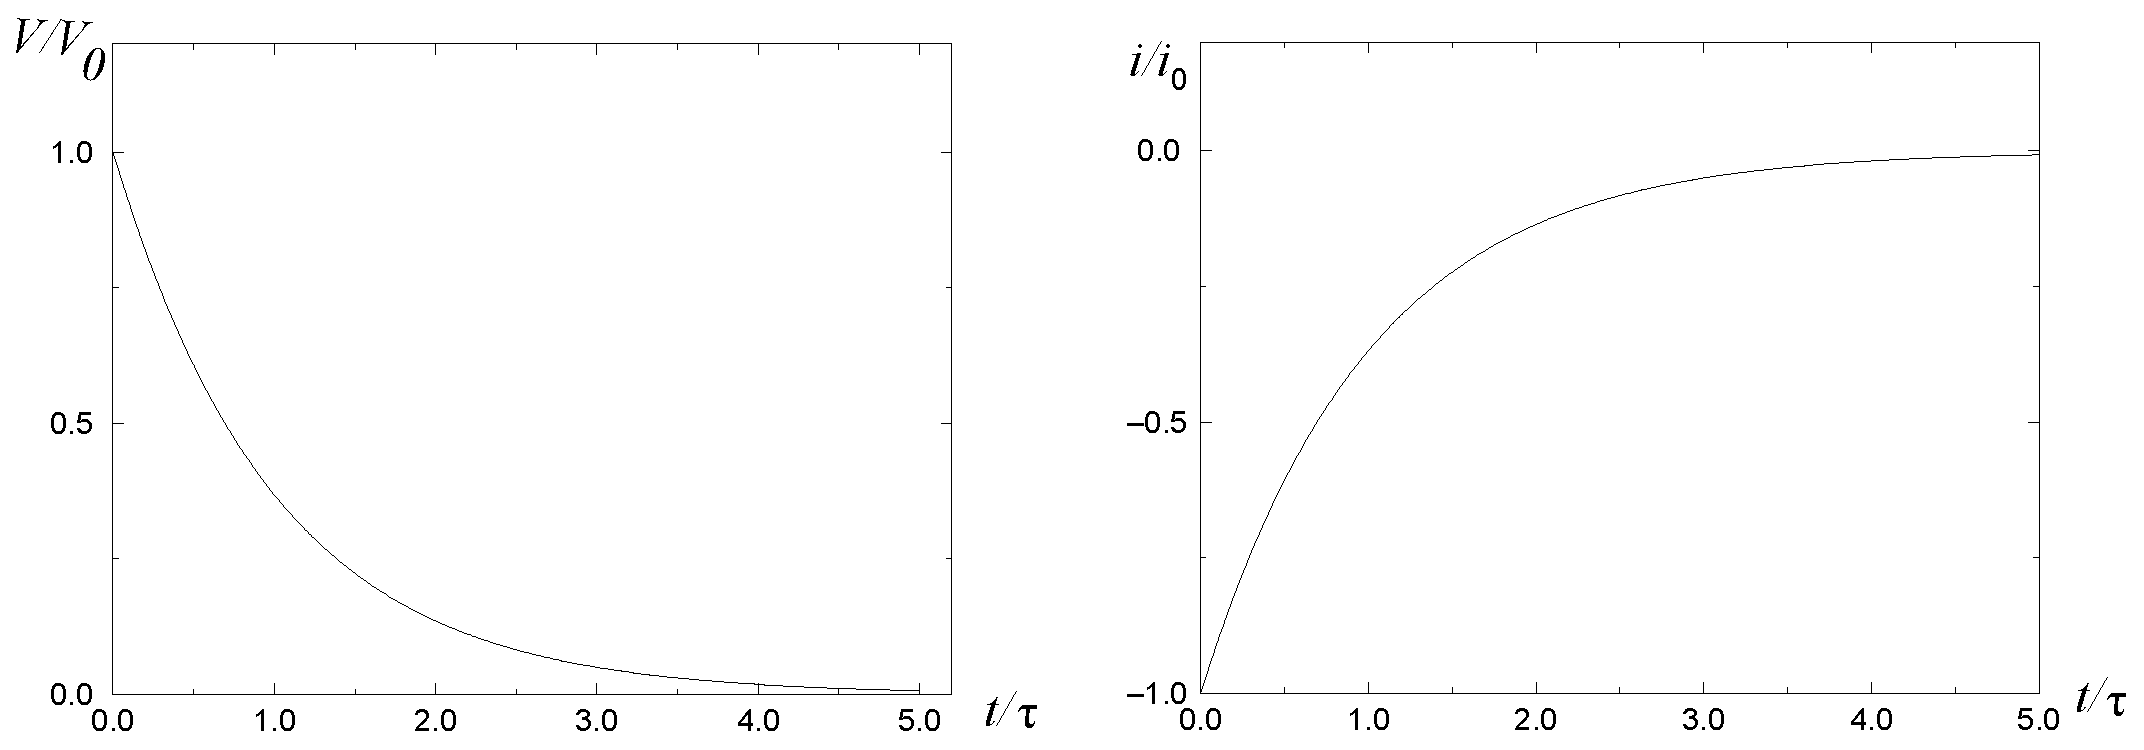
\includegraphics[scale=0.4]{5_rccircuits/dischargevi.eps}
\caption{Discharging voltage and current as functions of time.}
\label{fig:RC:dischargingiv}
\end{figure}

\subsection{AC Response of Capacitors}

Having seen that capacitors introduce a time scale into a system which 
otherwise had none (DC circuit), we want to examine how this intrinsic time
scale interacts with an AC circuit, one that has a natural period. To carry
this out, consider the circuit sketched in Figure 
\ref{fig:RC:driven rc circuit}. 
\begin{figure}[htb]
\centering 
\epsfxsize=8cm 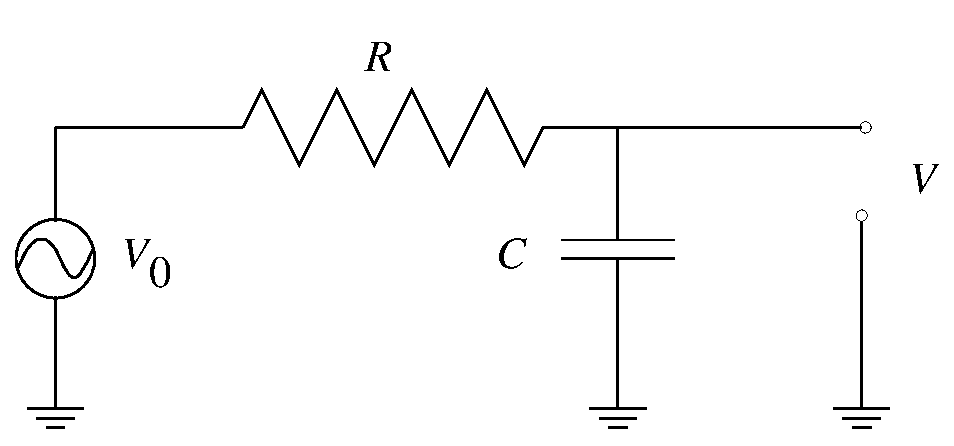
\includegraphics[scale=0.5]{5_rccircuits/rc2.eps}
\caption{A sinusoidally driven RC circuit.}
\label{fig:RC:driven rc circuit}
\end{figure}
Suppose the input voltage~$V$ oscillates with angular frequency~$\omega$; then
we can sum the voltage drops across the capacitor and the resistor and set that
equal to the oscillating voltage (Kirchoff's Law again). We find, just as 
before, that
\begin{eqnarray*}
V = V_C + V_R = \frac{Q}{C}+R\frac{dQ}{dt}
\end{eqnarray*}
Inserting $V = V_0 \sin (\omega t)$, we find that the charge on the capacitor 
obeys the relationship
\begin{eqnarray}
\frac{dQ}{dt} + \frac{1}{RC} Q = \frac{V_0}{R} \sin (\omega t).
   \label{eq:RC:oscillatingQ}
\end{eqnarray}
We can solve this differential equation using the same integrating factor
approach we employed in the DC case for charging the capacitor. The integrating
factor is the same, since the left-hand side is identical. After introducing 
this factor, equation (\ref{eq:RC:oscillatingQ}) becomes
\begin{eqnarray*}
\frac{d}{dt} \left( e^{t/\tau} Q \right) = \frac{V_0}{R} e^{t/\tau} \sin
(\omega t),
\end{eqnarray*}
where, of course, $\tau=RC$. Integrating both sides with respect to time and 
enforcing $Q=0$ when $t=0$ yields
\begin{eqnarray*}
Q(t) = \frac{V_0}{R} e^{-t/\tau} \int_0^t e^{t/\tau} \sin (\omega t) dt.
\end{eqnarray*}
You can evaluate the integral with a double application of integration by 
parts (Exercise!). The result is
\begin{eqnarray*}
Q(t) = \frac{V_0}{R} \frac{1}{1+(\omega \tau)^2} \left( \sin (\omega t) -
       \omega \tau \cos(\omega t) \right).
\end{eqnarray*}  
We can clean this result up by combining the trig functions using a phase 
angle. Consider the expansion
\begin{eqnarray*}
\sin(\omega t - \phi) = \sin(\omega t) \cos\phi - \cos(\omega t) \sin\phi.
\end{eqnarray*}
We can use this to find $\sin\phi$ and $\cos\phi$ by matching the corresponding
terms. We find initially that
\begin{eqnarray*}
\sin\phi = \omega \tau,\\
\cos\phi = 1,
\end{eqnarray*}
but these aren't compatible, since $\sin^2 \phi + \cos^2 \phi =1$. If we 
divide each by $\sqrt{1+(\omega \tau)^2}$ to force the Pythagorean identity, we
then see that
\begin{eqnarray*}
\sin\phi = \frac{\omega \tau}{\sqrt{1+(\omega \tau)^2}}\\
\cos\phi = \frac{1}{\sqrt{1+(\omega \tau)^2}}, 
\end{eqnarray*}
which are perfectly legal mathematical expressions. Thus, the phase angle can
be found from
\begin{eqnarray}
\tan \phi = \omega \tau.\label{eq:RC:phaseangle}
\end{eqnarray}
Incorporating this into the solution, we find that the charge on the capacitor
oscillates according to
\begin{eqnarray*}
Q(t) = Q_0 \frac{\sin(\omega t - \phi)}{\sqrt{1+(\omega \tau)^2}},
~~~\tan\phi=\omega\tau,    
\end{eqnarray*}
where $Q_0 = CV_0$, as usual. Using the same reasoning as in the DC analysis, 
we find the voltage across the capacitor $V$ and current in the circuit $i$ to 
be
\begin{eqnarray}
V(t) = \frac{Q(t)}{C} = V_0 \frac{\sin(\omega t - \phi)}
        {\sqrt{1+(\omega \tau)^2}}
       \label{eq:RC:oscillatingv}\\
i(t) = i_0\frac{\omega \tau}{\sqrt{1+(\omega \tau)^2}} 
       \cos(\omega t - \phi),
       \nonumber
\end{eqnarray}
where $i_0=Q_0/\tau$ as in the DC case. These relations are plotted as a 
function of time in Figure~\ref{fig:RC:oscillatingiv}. From these two 
relations, we find that the capacitor simply shifts the phase of oscillation 
and adjusts the amplitude according to the input frequency. This frequency
dependence forms the basis for sorting out signals base on frequency content. 
For the case we've analyzed here, the higher the frequency (large $\omega$) the
smaller the amplitude; so, this circuit functions as a low-pass filter, meaning
that lower frequencies can get through with only a slight phase shift, but 
higher frequencies are cut-off. 
\begin{figure}[htb]
\centering 
\epsfxsize=8cm 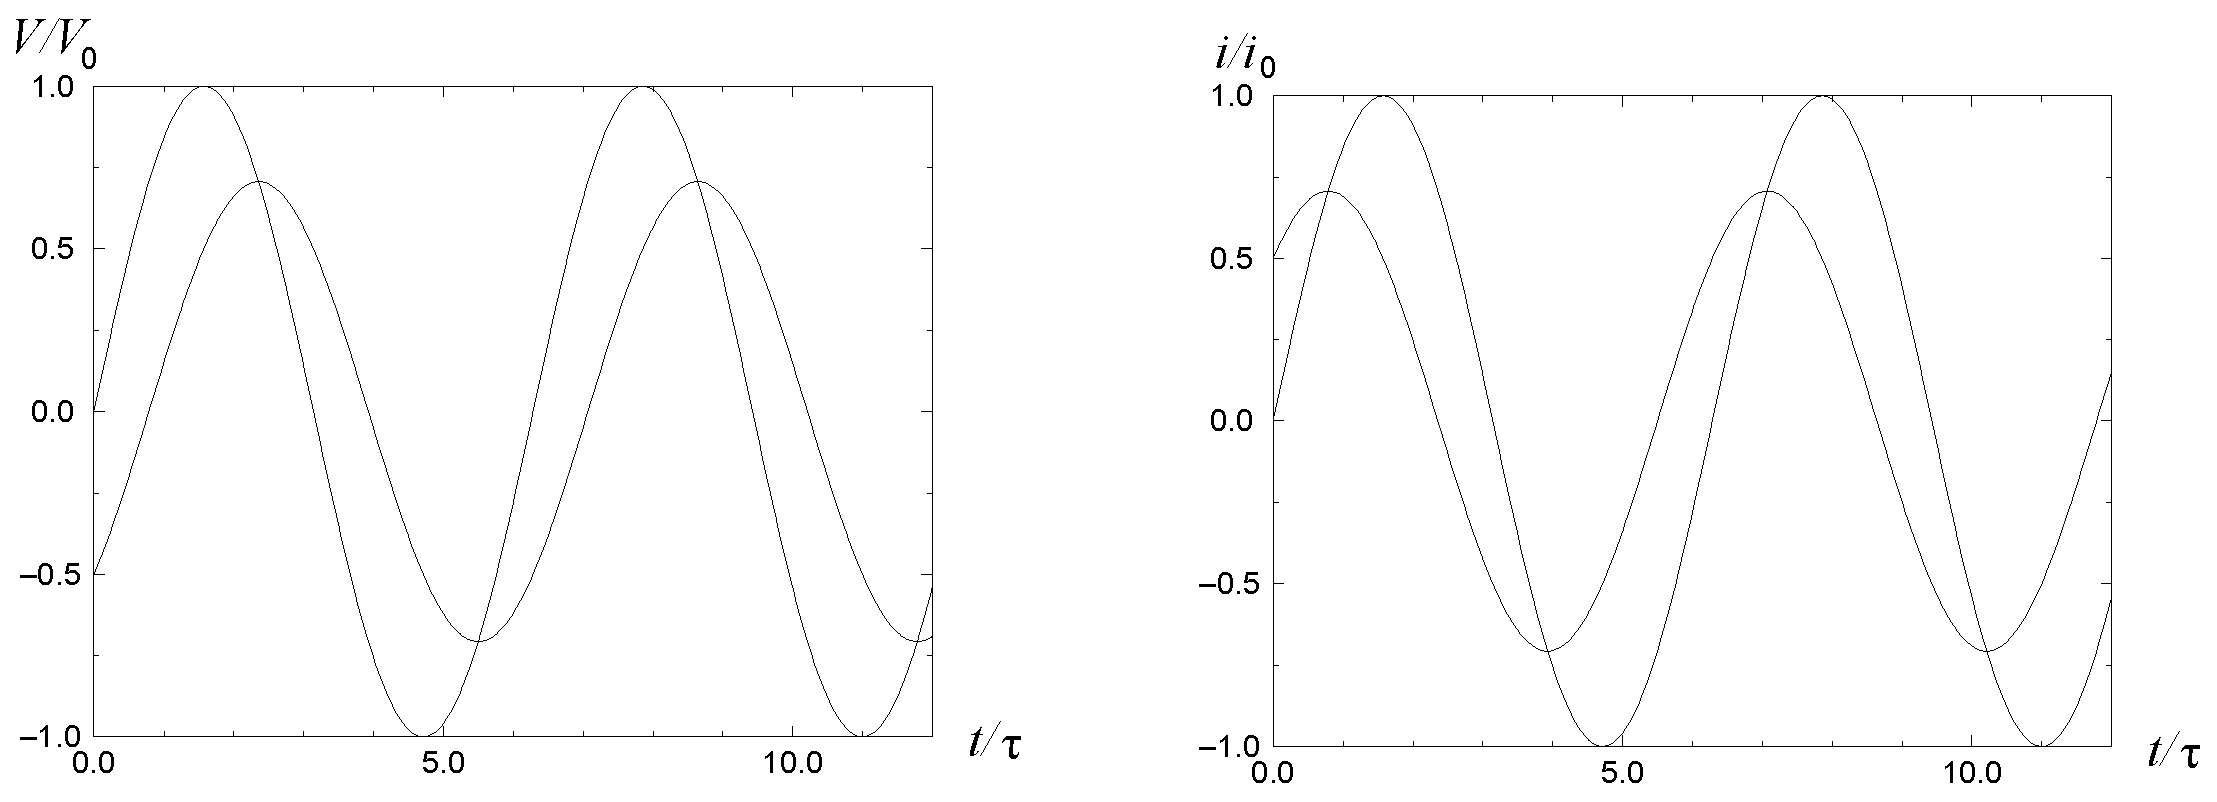
\includegraphics[scale=0.4]{5_rccircuits/sineviout.eps}
\caption{Voltage and current response of an RC circuit to a sinusoidal
input voltage with $\omega \tau = 1$.}
\label{fig:RC:oscillatingiv}
\end{figure}

You might ask, at what frequency does this filter start to really affect the 
signal? The answer to this question lies in the denominator of 
equation~\ref{eq:RC:oscillatingv}. The denominator is very close to $1$ for 
$\omega \ll 1/\tau$ and is very large for $\omega \gg 1/\tau$. Thus, we should
expect that for angular frequencies around $1/\tau$, the signal begins to
change. This value is called the {\em cutoff} angular frequency and is
typically denoted $\omega_c$. Thus, $\omega_c = 1/\tau$. To make this clearer,
consider the output amplitude, that is the stuff in front of the sine function
in equation~(\ref{eq:RC:oscillatingv}). We plot this function versus
normalized frequency in Figure~\ref{fig:RC:amplitude1}.
\begin{figure}[htb]
\centering 
\epsfxsize=10cm \includegraphics[scale=0.5]{5_rccircuits/campout.eps}
\caption{Voltage amplitude across the capacitor as a function of input 
frequency.}
\label{fig:RC:amplitude1}
\end{figure}
We see that, for frequencies below the cutoff, the amplitude is still above 
70\% that of the input signal. For frequencies above the cutoff, the amplitude 
decays rather slowly, dropping below 20\% for angular frequencies above about 
$5\omega_c$.

We have been discussing the voltage across the capacitor and we've found that
it is greatly suppressed for frequencies above the cutoff. If, on the other 
hand, we examine the voltage across the resistor, we find
\begin{eqnarray*}
V_R(t) = i(t)R = V_0 \frac{\omega \tau}{\sqrt{1+(\omega \tau)^2}}
         \cos(\omega t - \phi ).
\end{eqnarray*}
This voltage behaves quite differently, as a function of frequency, from the 
voltage across the capacitor. We plot its behavior in 
Figure~\ref{fig:RC:amplitude2}. For $\omega \ll 1/\tau$ the denominator is 
roughly $1$ while the numerator is small; so, the amplitude for low frequency 
waves is reduced compared to high frequency oscillations. For large 
frequencies, $\omega \gg 1/\tau$, the frequency dependence reduces to $
1$; hence, the amplitude of high frequency oscillations is unaffected by the 
circuit.
\begin{figure}[htb]
\centering 
\epsfxsize=10cm \includegraphics[scale=0.5]{5_rccircuits/rampout.eps}
\caption{Voltage amplitude across the resistor as a function of input 
frequency.}
\label{fig:RC:amplitude2}
\end{figure}  

We can understand the physical origin of these two different behaviors by 
examining what the capacitor actually does. If the input voltage is larger than
the voltage across the capacitor due the charge on its plates, then charge will
flow onto the plates, increasing the potential across them. Oppositely, when 
the driving voltage falls below that on the capacitor, charge flows off the plates, decreasing the potential. Thus, the voltage on the capacitor must 
{\em follow} the input voltage, leading to a phase shift in the output. This 
charging and discharging process takes place on the time scale defined by 
$\tau$. If the period of the input voltage oscillation is shorter than this
reaction time of the capacitor, a very small amount of charge has time to 
build up on the plates before its drained away again. This prevents the 
potential from growing large and cuts off the signal. On the other hand, if 
the period of the input oscillation is longer than $\tau$, then charge has 
time to build up on the plates, permitting the voltage to increase and allowing
the signal to pass. Since the voltage across the resistor is the input voltage
minus the voltage across the capacitor, it has the exact opposite behavior, but
with the same cutoff.

\section{Apparatus}

The major pieces of equipment we'll need to use in this lab have already been 
discussed in the oscilloscope lab. We will use the oscilloscope and frequency
generator, the breadboard and electrical components like resistors and 
capacitors. The only new item is the capacitor.

The capacitors we will use are electrolytic capacitors. Their plates have 
various shapes and are typically filled with a dielectric medium.
All of them have a nominal value of the capacitance inscribed on them somewhere.
%, which we will take as the actual value for the capacitance. 
Once we have measured the
time constant for a circuit with known resistance, we can then back out the 
capacitance and check the nominal value.  We note also that capacitors 
occasionally have an arrow or ring inscribed on them to denote the way they 
should be oriented in a circuit; the contact on the same side as the mark 
should be connected toward ground, see Figure~\ref{fig:rc:capacitor}.  
\begin{figure}[htb]
\centering 
\epsfxsize=9cm 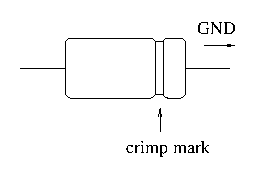
\includegraphics{5_rccircuits/capacitor.eps}
\caption{The marks which indicate the correct orientation of a capacitor.}
\label{fig:rc:capacitor}
\end{figure}

\clearpage

%  Label worksheets by \thechapter.W
\renewcommand{\thesection}{\thechapter.W}

\section{RC Circuits and Filters Worksheet}
{\bf \Large Name:}~ \rule{5cm}{.1mm}~~~~~~~
{\bf \Large Day/Time:}~\rule{3cm}{.1mm}\\
{\bf \Large Partner's Name:}~\rule{6cm}{.1mm}\\
 \subsection{In-Lab Procedure}

\subsubsection{DC Response}

Since most of the capacitors available to us have extremely small values of 
capacitance, typically on the order of $\mu$F, the time constants involved will
be small fractions of a second (usually ms). This makes it difficult to use a
multimeter to observe the voltage behavior during charging and discharging 
cycles. We will circumvent this problem by having the function generator act
as a high frequency switch. We will do this by using the square wave output to
toggle the circuit back and forth between the switch positions 1 and 2 in 
Figure~\ref{fig:RC:cap1}. When the square wave is low, this will act like the 
discharge phase (position 2), and when it is high, the circuit changes to 
position 1 and the capacitor charges. We can choose the frequency of this 
switching process to allow the capacitor to completely charge and completely 
discharge and then repeat. We can then use the oscilloscope to examine the time
dependence of the voltage in each case. In Figure~\ref{fig:RC:onoff} we show 
what the typical input and output voltages should look like. \\
\begin{figure}[htb]
\centering 
\epsfxsize=10cm 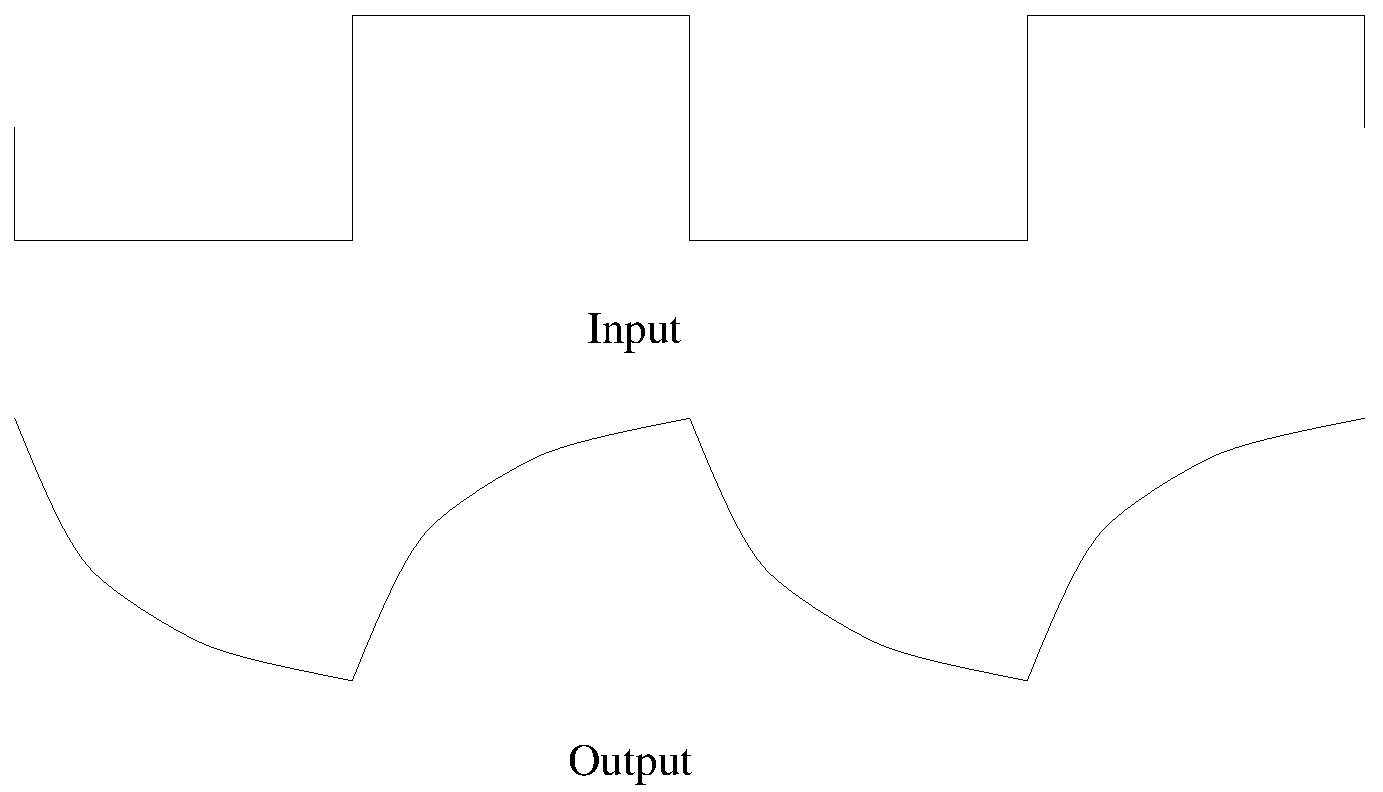
\includegraphics[scale=0.5]{5_rccircuits/squareout.eps}
\caption{RC circuit response to a square wave input.}
\label{fig:RC:onoff}
\end{figure}

\noindent Using the given capacitor and small resistor, 
construct the circuit
shown in Figure~\ref{fig:wiring} with the function generator acting as the
switch. Measure the provided resistor as well as the capacitance of your capacitor
with the multimeter and record its value, with uncertainties, below:
\begin{center}
$R_{meter}=$~ \rule{3cm}{.1mm}~~~~
$C_{meter}=$~ \rule{3cm}{.1mm} \\
\end{center}
\noindent Set the function generator to provide a square wave output 
and choose an initial frequency of about 1~kHz. Split the signal coming out of 
the function generator, sending one to your circuit and the other to Channel~1
of the oscilloscope; trigger on Channel~1. 
We will use the T-connectors to split the output of the function generator, as
illustrated in Figure~\ref{fig:wiring}.
\begin{figure}[htb]
\epsfxsize=15cm
\centering 
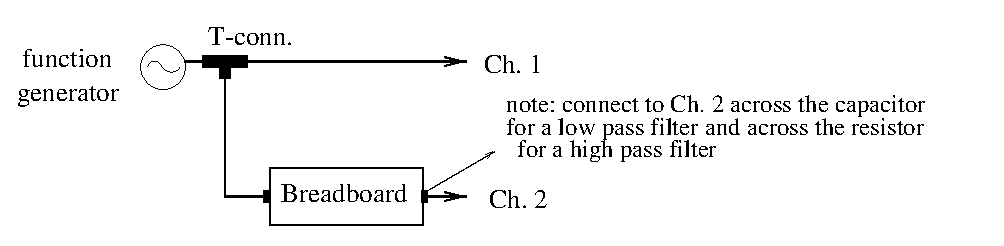
\includegraphics[scale=0.8]{5_rccircuits/wiring.eps}
\caption{We will use the T-connector and trigger the oscilloscope on 
channel~1.}
\label{fig:wiring}
\end{figure}
The split signal will allow us to trigger on the raw output of the
function generator (on channel~1). We will use a 51~k$\Omega$ resistor and a
3.3~nF capacitor in our RC~circuit.
%Since the function generator has a {\bf 50~$\Omega$ output impedance}, 
%what should really go into our formulae during our analysis is the 
%{\bf equivalent resistance  of each circuit}. Take care when evaluating this,
%since the resistor and the function generator can be in series or in parallel,
%depending on where you decide to make measurements.
What we will set up on the board is illustrated in Figure~\ref{fig:rcboard}.

\noindent Arrange the circuit in Figure~\ref{fig:rcboard} on 
the breadboard and set the 
function generator to provide a square wave at about 1~kHz.  Connect the 
alligator clips of the BNC-to-alligator clip wire to jumpers on the board 
so that they are measuring the voltage across the {\it capacitor}, $V_C$; 
send this into channel~2 of the oscilloscope. \\
\ \\
\clearpage
\begin{figure}[htb]
\epsfxsize=15cm
\centering 
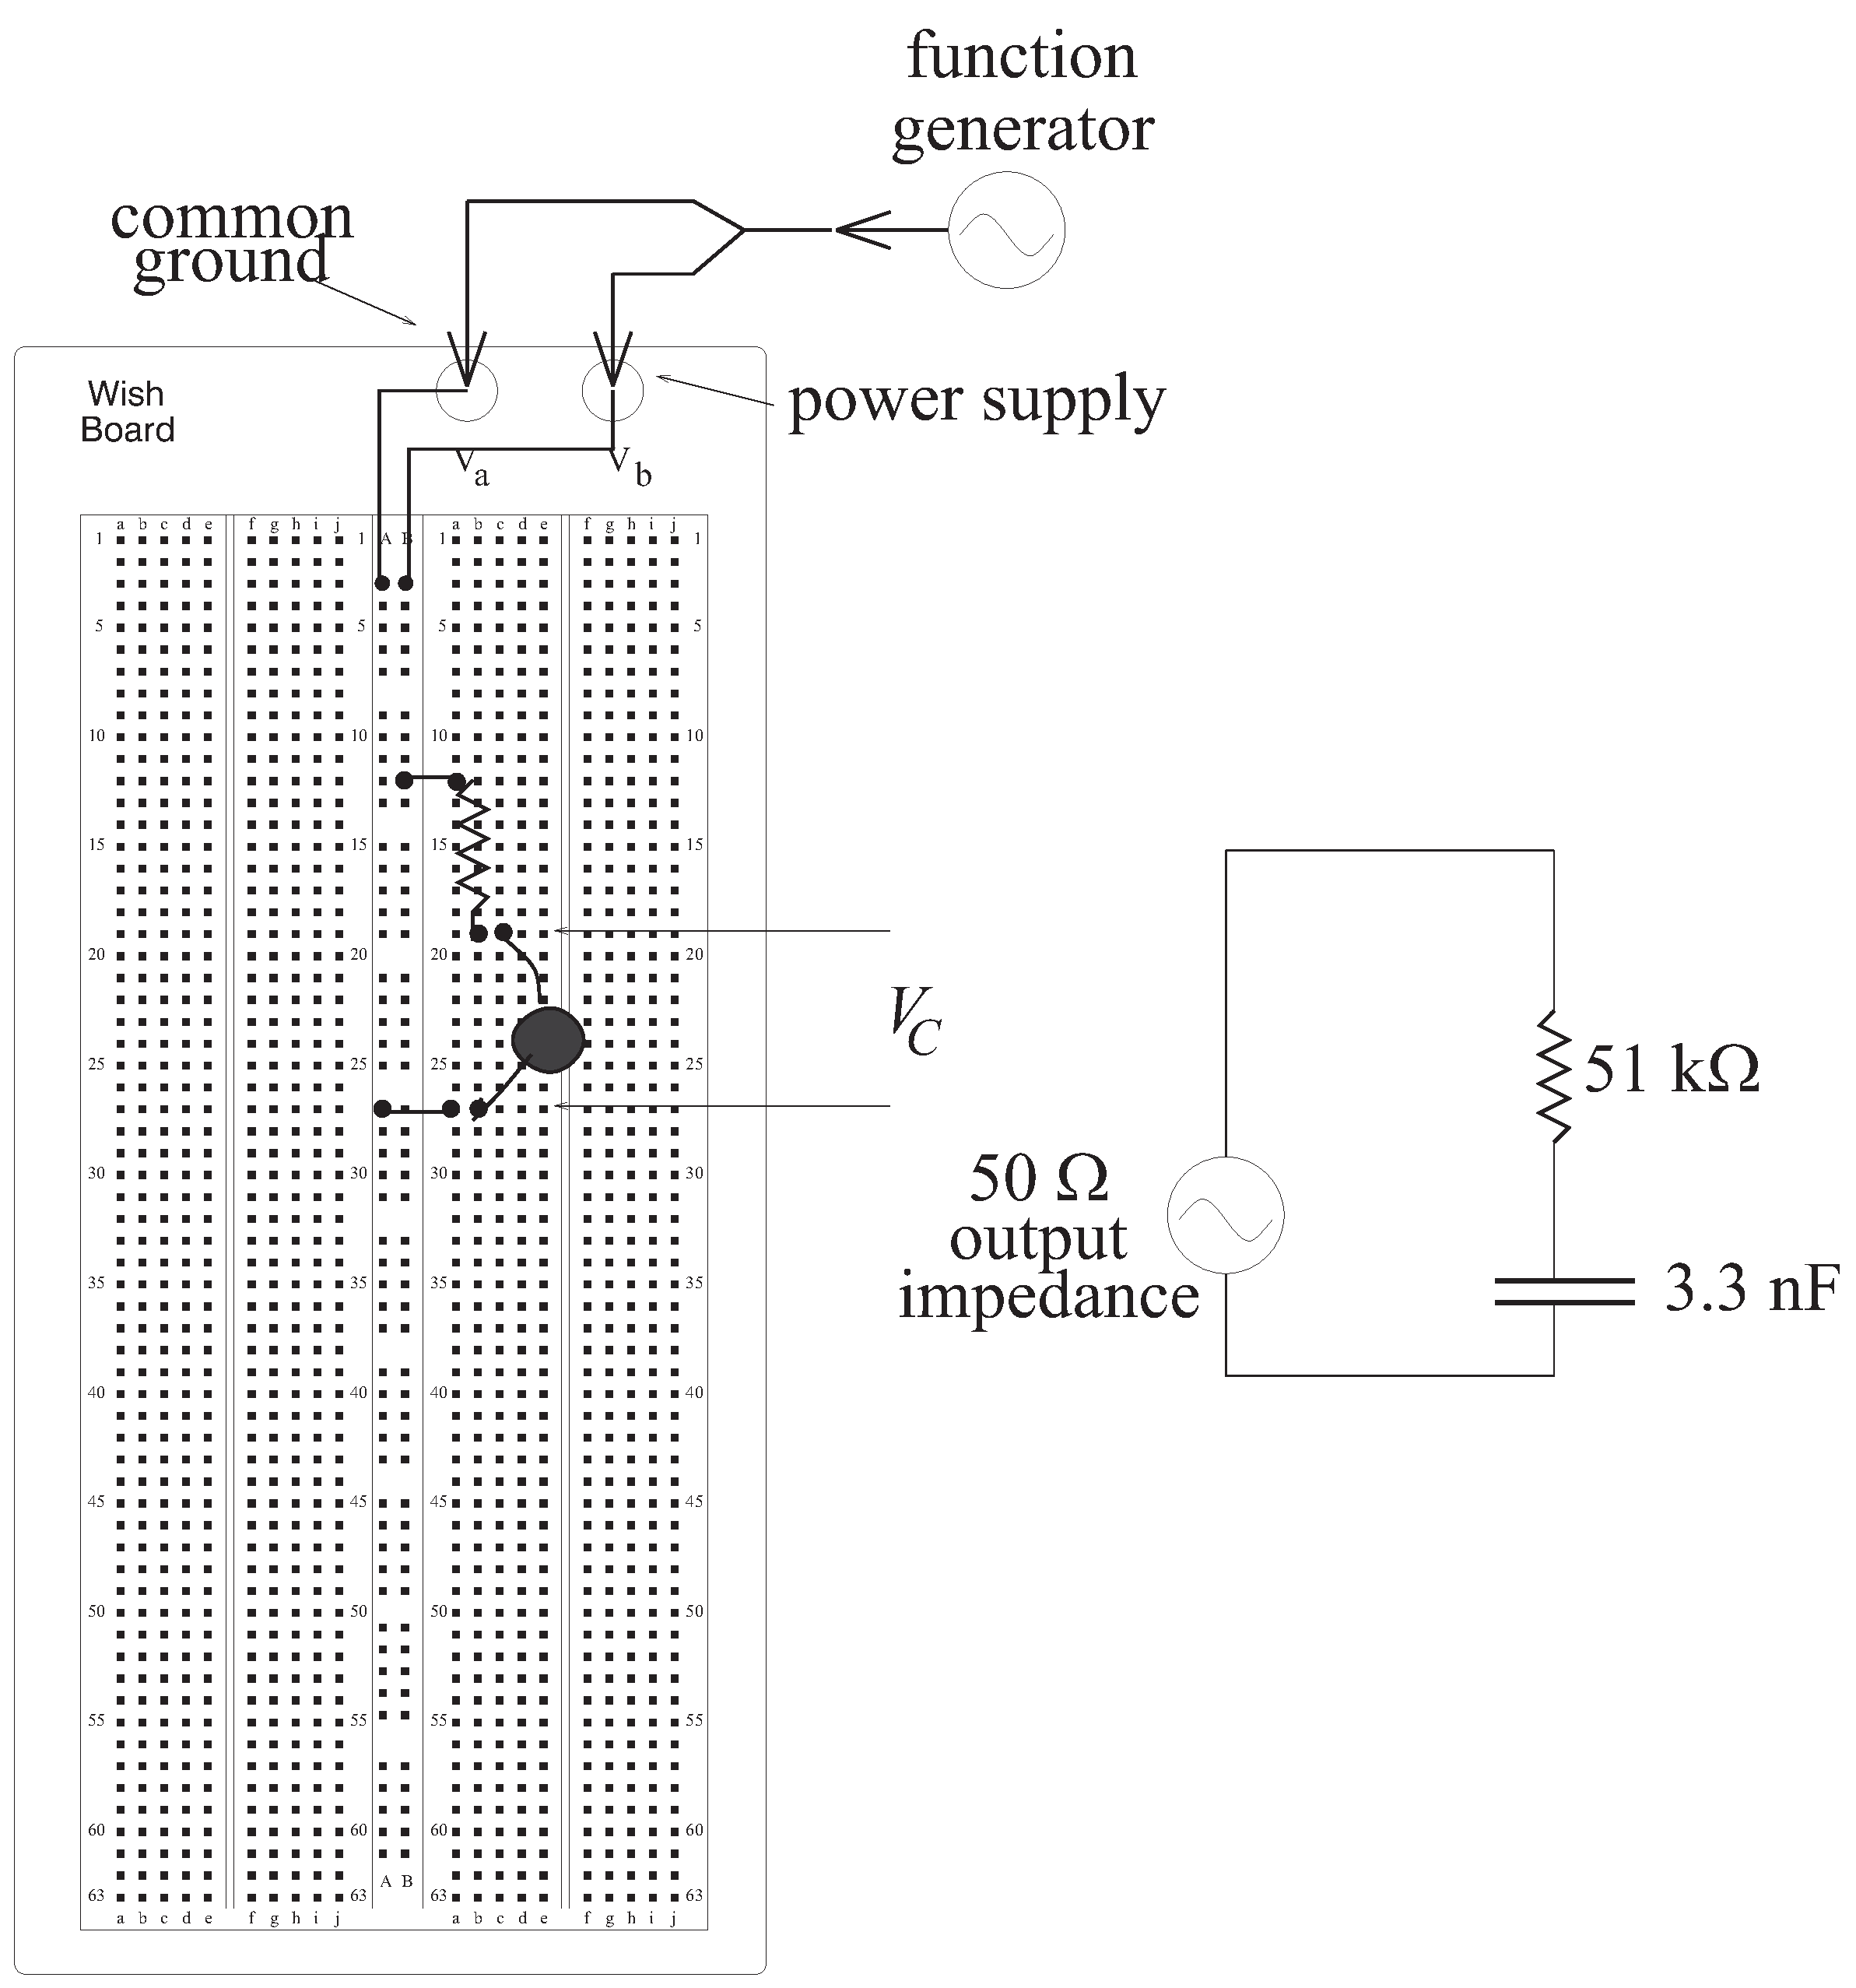
\includegraphics[scale=0.4]{5_rccircuits/rcboard.eps}
\caption{The proper breadboard connections for our RC circuit. Note that the
circuit can be configured so that the oscilloscope measures the voltage across
the capacitor ($V_C$) or across the resistor ($V_R$).} 
\label{fig:rcboard}
\end{figure}

\clearpage

\noindent Trigger the oscilloscope on 
channel~1 and display channel~2; adjust the scope until
you can see the decay/growth response illustrated as ``output'' at the bottom
of Figure~\ref{fig:RC:onoff} in the manual.  By adjusting the V/div and
sec/div knobs of the scope, focus in on a {\it decay} portion of the signal. Adjust the channel~2
vertical position and the horizontal position knobs until the maximum of the 
decay curve lands on a vertical grid line (voltage axis) and the minimum lands 
on a horizontal grid line (time axis), as illustrated in 
Figure~\ref{fig:scope}. \\

\begin{figure}[htb]
\epsfxsize=8cm
\centering 
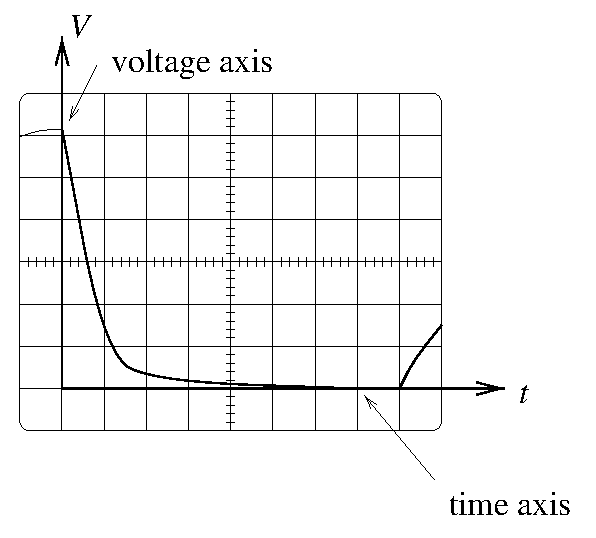
\includegraphics[scale=0.7]{5_rccircuits/scope.eps}
\caption{Adjust the scope until you have the decay curve aligned with a 
``voltage axis'' and ``time axis.''}
\label{fig:scope}
\end{figure}

\noindent Now use the axes you thus created to measure the voltage-time pairs.
Adjust the oscilloscope to observe the discharging phase; 
use the scale 
settings to focus the display in on one of the decay portions of the output
signal. You can now read off the discharge voltage as a function of time. Take 
ten voltage-time pairs and enter the voltage-time pairs into 
Table~\ref{tab:RC:decay}.
{\bf Take Note:} Your first measurement should be of the 
voltage at the beginning of
the discharging phase. (That's the peak of the curve on the screen.) 

\begin{table}[htb]
\begin{center}
\begin{tabular}{|c|c|c|c|c|}
\hline
\multicolumn{5}{|c|}{Voltage and Time Coordinates} \\
\hline
Voltage & Time & & Voltage & Time \\
\hline
\hspace*{3cm} & \hspace*{3cm} & \hspace*{.1cm} & \hspace*{3cm} & \hspace*{3cm} \\
& & & & \\
\hline
& & & & \\
& & & & \\
\hline
& & & & \\
& & & & \\
\hline
& & & & \\
& & & & \\
\hline
& & & & \\
& & & & \\
\hline

\end{tabular}
\end{center}
\caption{V vs. t measurements for discharging capacitor.}
\label{tab:RC:decay}
\end{table}


\subsection{In-Lab Computer Work}
According to 
equation~(\ref{eq:RC:discharge voltage}), the quantity $\ln (V/V_0)$ should be 
linearly related to $t$. What's $V_0$ in this case? \\
\begin{center}
$V_0 = $ ~ \rule{3cm}{.1mm} \\
\end{center} 
Graph $\ln (V/V_0)$ versus 
$t$ with the set of data contained in Table~\ref{tab:RC:decay} with 
Kaleidagraph.  You must calculate the uncertainty in $\ln (V/V_0)$.  Remember
that both $V$ and $V_0$ have uncertainties associated with them.
Calculate $\Delta\ln (V/V_0)$ below.
Remember that the computer will do most of the work for you.  Just do {\bf one
sample calculation} and then use the computer.  {\bf SHOW WORK.} \\
\vspace*{2.3cm} \\
\begin{center}
$\Delta\ln (V/V_0)$  ~ \rule{3cm}{.1mm} \\
\end{center}

\noindent  Find the slope and intercepts with uncertainties and 
record their values in Table~\ref{tab:RC:slope1}. 
\begin{table}[htb]
\begin{center}
\begin{tabular}{|c|c|}
\hline
\multicolumn{2}{|c|}{RC Circuit} \\
\hline
Slope & Intercept \\
\hline
\hspace*{5cm} & \hspace*{5cm} \\
& \\
\hline
\end{tabular}
\end{center}
\caption{Slope and Intercept for the resistor $ln(V/V_0)$ vs.\ $t$ plot.}
\label {tab:RC:slope1}
\end{table}

\noindent From equation~(\ref{eq:RC:discharge voltage}),
 determine how the slope of your plot should be
related to the time constant of your circuit. With this information, 
calculate the time constant of your circuit, 
$\tau _{meas}$, and its uncertainty from the slope of your plot. \\
\vspace*{2cm} \\
\begin{center}
 $\tau_{meas}$ = ~ \rule{3cm}{.1mm} \hspace*{1cm} $\Delta(\tau_{meas})$ = ~ \rule{3cm}{.1mm} \\
\end{center}
\subsection{In-Lab Procedure}
\subsubsection{AC Response}
Now adjust the function generator to provide a sinusoidal input to the circuit.
Referring to the circuit diagram in Figure~\ref{fig:lowpass} for this 
arrangement. 
\begin{figure}[htb]
\epsfxsize=8cm
\centering 
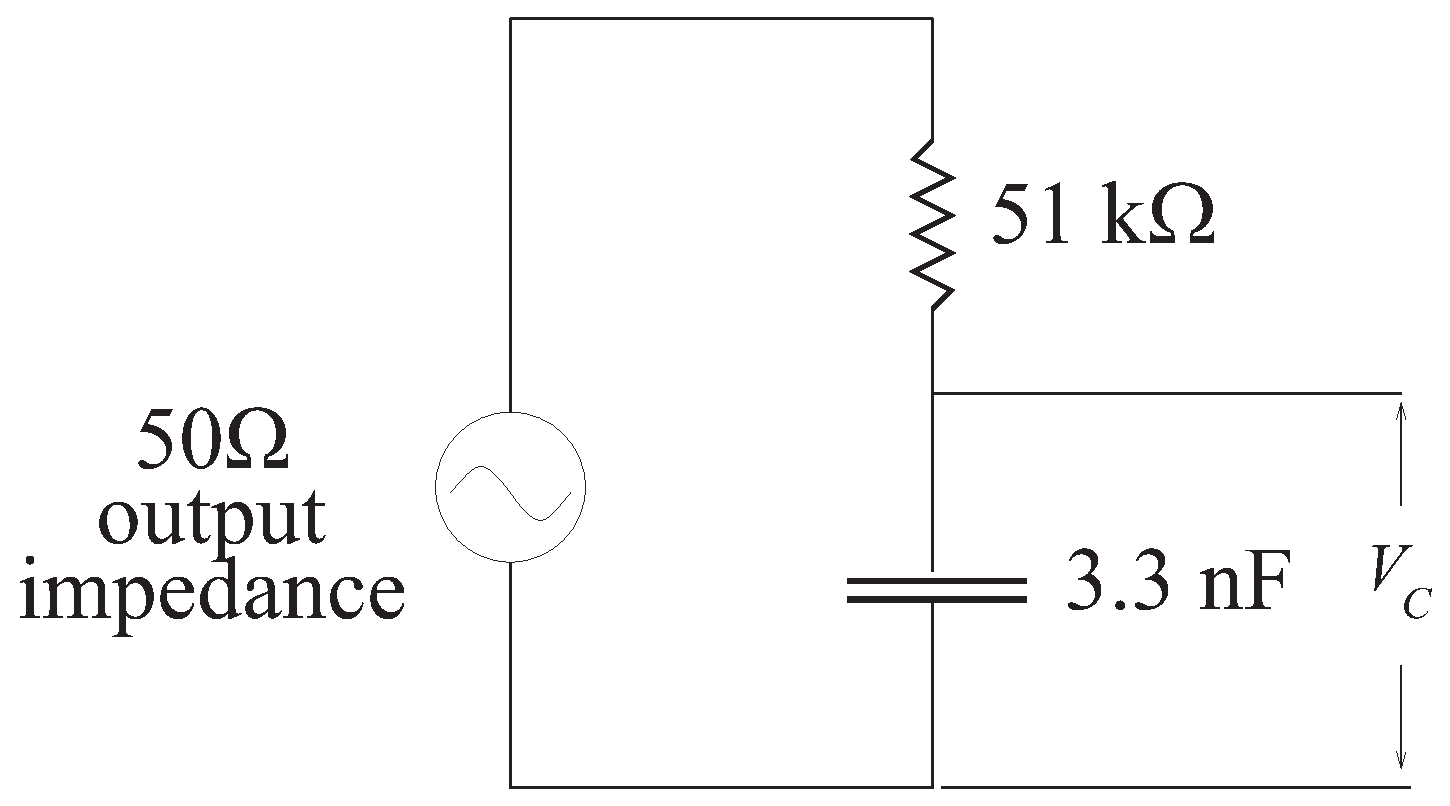
\includegraphics[scale=0.35]{5_rccircuits/lowpass.eps}
\caption{A low-pass filter arrangement.}
\label{fig:lowpass}
\end{figure}
\noindent Use $\tau _{meas}$ to determine the natural cutoff frequency of your
circuit (without uncertainty).
Record this value and {\bf Show work}:
\vfill
\begin{center}
$f_c=$~ \rule{3cm}{.1mm}
\end{center}
\newpage 
\noindent Set the function generator to a 
frequency below the cutoff. You can tell that you're below the cutoff when you 
see that the amplitude of the output signal doesn't depend on the frequency;
this will probably be somewhere in the 1~kHz range of the function generator.
Set the function generator to about this frequency and compare the oscilloscope
screen with Figure~\ref{fig:RC:oscillatingiv}. 
Next, switch the oscilloscope to display only channel two and set the frequency
generator to a frequency below the cutoff. Measure the peak-to-peak amplitude of the output
waveform as a function of the frequency for ten different frequencies. \\

\noindent {\bf Make sure that most of your frequency values extend 
past the cutoff.}
Remember that you should always measure your frequencies from the periods of 
the waves on the oscilloscope.  Enter your amplitude-period pairs into
Table ~\ref{tab:RC:lowpass}.  {\bf Take Note:}
\begin{enumerate}
 \item Your first amplitude measurement should be taken from
a signal with a frequency of around {\bf 100 Hz}. 
 \item Take data at your cutoff frequency $f_c$. You will compare that value to the theoretical value later.
 \item A good majority (at least seven) of your amplitude
measurements should be taken from signals with frequencies {\it above}
the natural cutoff frequency of the circuit.
 \item Once you have taken this measurement, DO NOT adjust the amplitude knob on the function
generator.
\end{enumerate}

\begin{table}[htb]
\begin{center}
\begin{tabular}{|c|c|c|c|c|c|c|}
\hline
\multicolumn{7}{|c|}{Amplitude vs. Period Measurements} \\
\hline
Amplitude & Period & $f$ &  & Amplitude & Period & $f$ \\
\hline
\hspace*{1.5cm} & \hspace*{1.5cm} & \hspace*{1.5cm}& \hspace*{.1cm} & \hspace*{1.5cm} & \hspace*{1.5cm}& \hspace*{1.5cm} \\
& & & & & & \\
\hline
& & & & & & \\
& & & & & & \\
\hline
& & & & & & \\
& & & & & & \\
\hline
& & & & & & \\
& & & & & & \\
\hline
& & & & & & \\
& & & & & & \\
\hline

\end{tabular}
\end{center}
\caption{Amplitude vs. Period Measurements.}
\label{tab:RC:lowpass}
\end{table}


\subsection{In-Lab Computer Work}
Now, plot the amplitude, $A_{exp}$, versus the frequency $f$ 
with error bars using the amplitude values from Table~\ref{tab:RC:lowpass} and calculating frequency from
the period values in Table~\ref{tab:RC:lowpass}.  Show a sample
calculation of $f$ and $\Delta f$ here. \\

\subsection{In-Lab Procedure}
\subsubsection{High-pass Filter}
Now reconfigure your circuit to measure the voltage across the resistor
by switching the position of the resistor and capacitor in your
circuit and connecting the clips to the oscilloscope across the resistor. Scan
the frequency across the cutoff and describe the behavior of the amplitude 
that you observe. You do not need to take any data here; just verbally express
what you observe.  \\
\ \\
\noindent {\bf Question 1:} Is this consistent with our predictions for a high 
pass filter? Why? \\
\vspace*{1.5cm} \\
\noindent {\bf Question 2:}  Estimate the cutoff
frequency and compare it to the cutoff frequency for the voltage across the 
capacitor. \\
\vspace*{2.2cm} \\
{\bf Question 3:} Does this make sense?  \\
\ \\


\subsection{Pre-Classroom Check List}
\noindent $\bigcirc$ \hspace*{1cm} Table~\ref{tab:RC:decay} completed with units and uncertainties \\
$\bigcirc$ \hspace*{1cm} Table~\ref{tab:RC:slope1} completed with units and uncertainties \\
$\bigcirc$ \hspace*{1cm} Table~\ref{tab:RC:lowpass} completed with units and uncertainties \\
$\bigcirc$ \hspace*{1cm} Plot of $ln(V/V_0)$  vs. $t$ labeled completely and correctly \\
$\bigcirc$ \hspace*{1cm} Plot of $A_{exp}$ vs. $f$ labeled completely and correctly \\
$\bigcirc$ \hspace*{1cm} Each student has her/his own plots and worksheet \\
 

\subsection{In-Classroom Calculations \& Analysis}

\subsubsection{DC Response}
From the measured values of the resistance and the capacitance of your circuit,
calculate the expected time constant,
$\tau _{calc}$. Record this below. Be sure to include units and uncertainties.
{\bf Show your work.}\\
\vspace*{0.5cm} \\
\begin{center}
$\tau _{calc}=$~ \rule{3cm}{.1mm} 
\end{center}

\noindent
From $\tau _{meas}$, and the measured resistance of your circuit, $R_{meter}$,
calculate a value for the capacitance of your circuit, $C_{meas}$. Record this
below. Be sure to include units and uncertainties. {\bf Show your work}.\\
\vspace*{0.5cm}
\begin{center}
$C_{meas}=$~ \rule{3cm}{.1mm} 
\end{center}
%\clearpage
\noindent Explain how equation~(\ref{eq:RC:discharge voltage}) in the lab 
manual leads you to expect a plot of ln($V/V_0$)
versus $t$ to be linear.
\vspace*{3cm}

\noindent 
Determine the expected value of the intercept of your plot and then compare 
this with the actual intercept value from your plot.
\vspace*{2cm}

\noindent
Compare the value of the circuit's time constant that you obtained
from the plot ($\tau _{meas}$), to its expected value ($\tau _{calc}$).
\vspace*{3cm}

\noindent
Compare the value of the capacitance from the measured time constant ($C_{meas}$),
with its value measured by the multimeter ($C_{meter}$).
\vspace*{3cm}

\subsubsection{AC Response}  

With the equation below, calculate $A_{theo}$ at the cutoff frequency $f_c=1/(2 \pi \tau_{meas})$, with uncertainty.\\
$$ 
A_{theo} = \frac{A_{in}}{\sqrt {1+(2\pi f \tau_{meas})^2} }.  
$$
\noindent Use the amplitude at $f=100 \, \mathrm{Hz} $ for the input amplitude $A_{in}$.\\

\noindent Compare your measured amplitude $A_{meas}$ at $f_c$ to 
$A_{theo}$ at $f_c$. To do this, you need to  discuss the
degree to which they agree within uncertainties.  
Show all your work. \\
\vspace*{3cm}
\clearpage
\subsection{Conclusion}

Write a {\it brief} (that is, a one or two paragraph) conclusion for
this lab below. In it, you should summarize the physical
principles which were meant to be illustrated in this experiment. You
should also describe the degree to which your data supported these
principles.

\vfill
\noindent Attach plots to the worksheet. \\
\ \\
{\Large End Worksheet} 
 

% Go back to ordinary section numbering
\renewcommand{\thesection}{\thechapter.\arabic{section}}
